%\documentclass[11pt]{article}

\documentclass[addpoints,12pt]{exam}

\usepackage[margin=2.5cm]{geometry}
\usepackage{graphicx}
\usepackage{listings}
\usepackage{xpatch}
\usepackage{color}
\usepackage{amsmath}
\usepackage[utf8]{inputenc}

\makeatletter
\xpretocmd{\item@points@pageinfo}{\normalfont}{}{}
\xapptocmd{\item@points@pageinfo}{\bfseries}{}{}
\makeatother

\begin{document}
	\begin{center}
		\LARGE\scshape{Fluorescencia}
		
		\vspace{1cm}
		\large\scshape{Juan Barbosa - 201325901}
	\end{center}

	La microscop\'ia de fluorescencia es una importánte técnica de microscop\'ia ya que permite observar objetos diminutos con gran magnificación y resolución. En el caso de la fluorescencia no se usa luz transmitida sino luz reflejada (o luz emitida por la muestra).
	
	\begin{figure}[h]
		\centering
		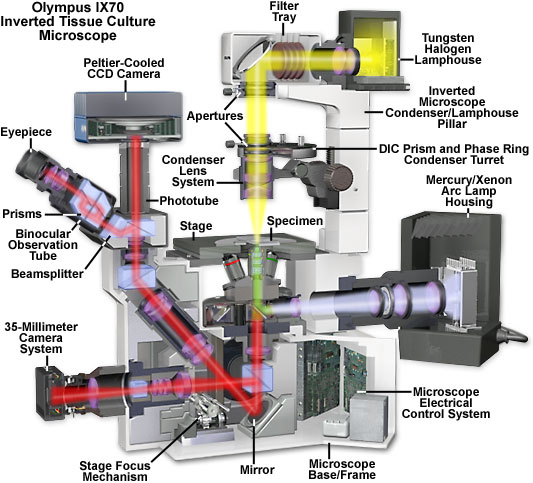
\includegraphics[width = 0.5\linewidth]{lightpaths.jpg}
	\end{figure}
	
	El esquema general del camino óptico de un microscópio de fluorescencia se muestra en la figura anterior. Un haz de luz se hace insidir sobre un filtro pasa bandas, el cual se conoce como el filtro de excitación. Posteriormente el haz pasa por el espéjo dicrócico, el cual refleja y transmite longitudes de onda específicas. Parte de la luz va en dirección en direcci\'on a la muestra, donde la luz incidente excita los fluor\'oforos en la muestra. Estos pueden ser propios de la muestra (autofluorescencia) o tintes agregados a la misma. La luz emitida pasa atrav\'es del dicr\'oico hasta alcanzar el filtro de emisi\'on, el cu\'al permite limitar la cantidad de fluor\'oforos detectados. Finalmente la luz llega al ocular, o a una c\'amara CCD.
	
	\begin{questions}
		{\question Qu\'e es un filtro de densidad neutra}
		
		Los filtros de densidad neutra son filtros que reducen la intensidad de la luz de forma homog\'enea para todas las longitudes de onda de la luz incidente.
		
		{\question Para qu\'e la apertura num\'erica est\'a optimizada para la c\'amara si se considera un factor de muestreo de 3?}
		
		En el datasheet se especifica que el tama\~no de los pixeles es de 6.45 x 6.45 $\mu$m. En una ccd la luz se proyecta sobre el plano de los pixeles. Existen dos posibles efectos en la proyecci\'on, por un lado es posible que demasiados pixeles contengan al mismo punto de Airy, lo cual implica informaci\'on redundante. En el caso opuesto cada pixel tendr\'a la informaci\'on de varios c\'irculos de Airy, lo cual no permite resolver los detalles.
		
		El tama\~no de la proyecci\'on ser\'a entonces:
		\begin{equation}
			P = \left(\dfrac{1.22\lambda}{2NA}\right)M \qquad \text{M: magnificaci\'on, NA: apertura num\'erica}
		\end{equation}
		
		La idea es que el tama\~no de la proyecci\'on sea de 3 pixeles:
		\begin{equation}
			\left(\dfrac{M}{NA}\right) \approx \dfrac{3(6.45)}{0.244} \approx 60 \qquad \text{con $\lambda = 500$ nm}
		\end{equation}
		
		{\question Cubo de filtros}
		\begin{table}[h]
			\centering
			\begin{tabular}{c|cccc}
				\hline
				\textbf{Molécula} & \textbf{1} & \textbf{2} & \textbf{5} & \textbf{6} \\
				\hline
				Alexa Fluor 488 & & X & & \\
				Mito Tracker & & X & X & \\
				DAPI & X & & & \\
				\hline
			\end{tabular}
		\end{table}
	\end{questions}

	A nivel de laboratorio la calibración del microscópio se realiza usando una guía de escala, para la cual cada línea representa 10 $\mu$m. Usando \texttt{ImageJ} se mide la distancia entre dos líneas grandes (100 $\mu$m), usando la función \texttt{Analyze->Set scale...} se determina la escala. El campo observado corresponde entonces con 441 x 333 $\mu$m.
	\begin{figure}[h]
		\centering
		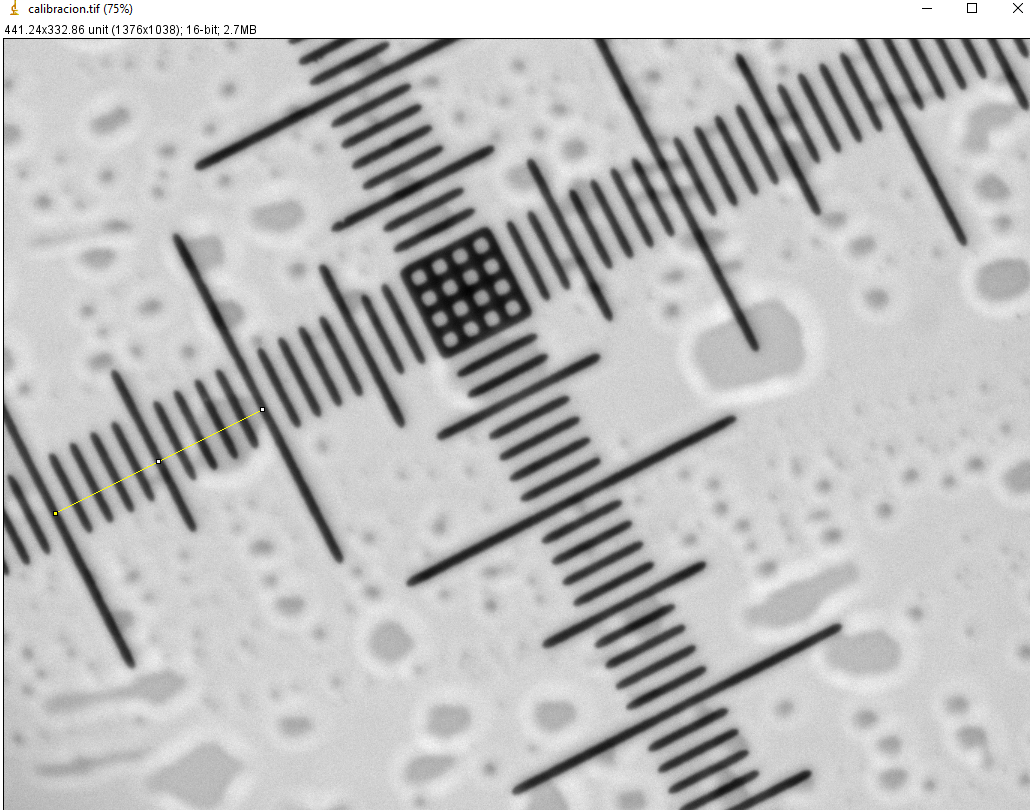
\includegraphics[width=0.7\linewidth]{calibracion.png}
	\end{figure}

	La combinación de los cromóforos da lugar a tres tipos distintos de tinción en las estructuras celulares. La superposición de las imágenes se da de la siguiente manera:
	\begin{table}[!h]
		\centering
		\begin{tabular}{cc}
			\hline
			\textbf{Imagen} & \textbf{Canal} \\
			\hline
			Image\_2567 & Rojo \\
			Image\_2570 & Verde \\
			Image\_2573 & Azul \\
			\hline
		\end{tabular}
	\end{table}

	Usando la escala es posible calcular el tamaño de los núcleos celulares, los cuales tienen forma ovalada con semieje menor de $4.88$ $\mu$m, y semieje mayor de $7.03$ $\mu$m.
	\begin{figure}[!h]
		\centering
		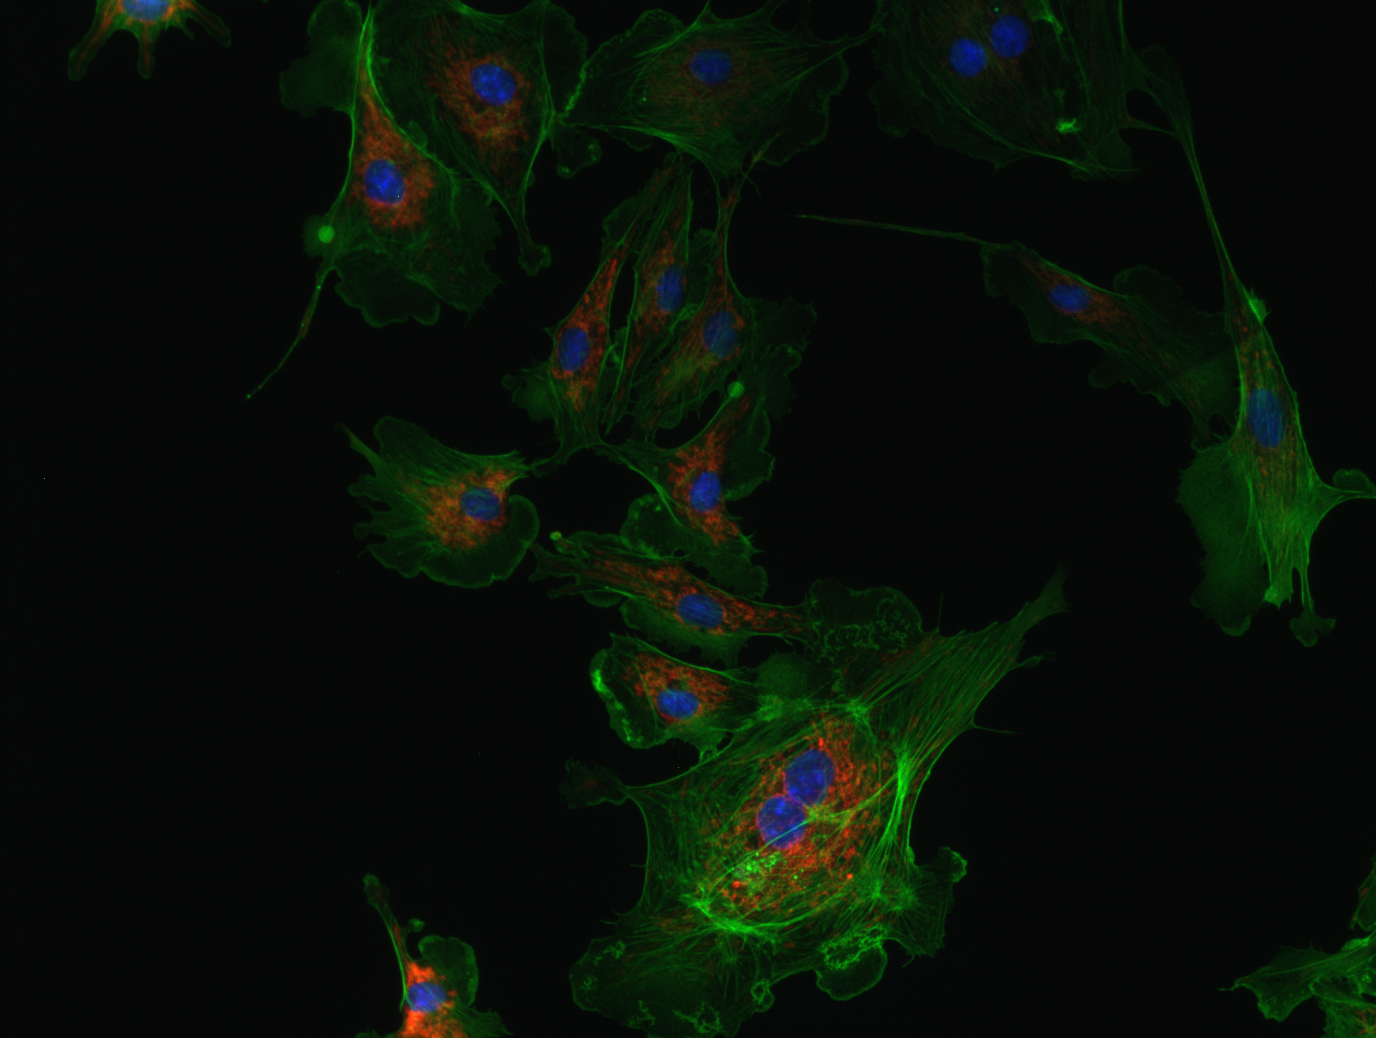
\includegraphics[width=0.7\linewidth]{composite.png}
	\end{figure}

	Finalmente se toman varias fotografías usando distintos tiempos de exposición con el objetivo de observar la importancia del rango dinámico de la cámara.
	
	\begin{figure}[!h]
		\centering
		\begin{tabular}{ccc}
			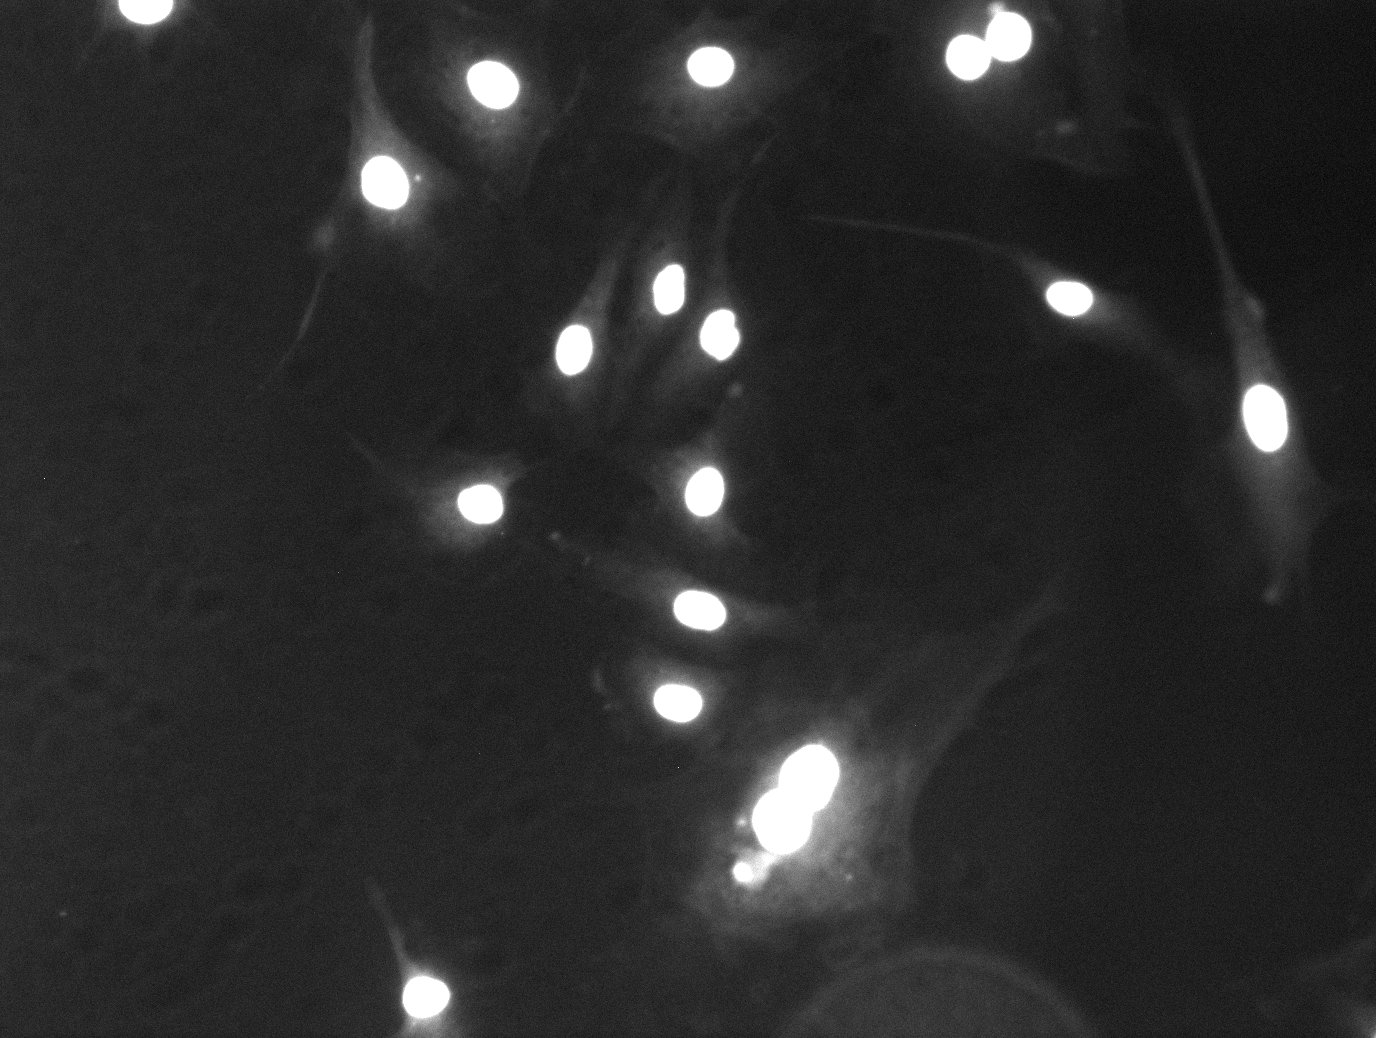
\includegraphics[width = 0.3\linewidth]{Image_2571.jpg} &
			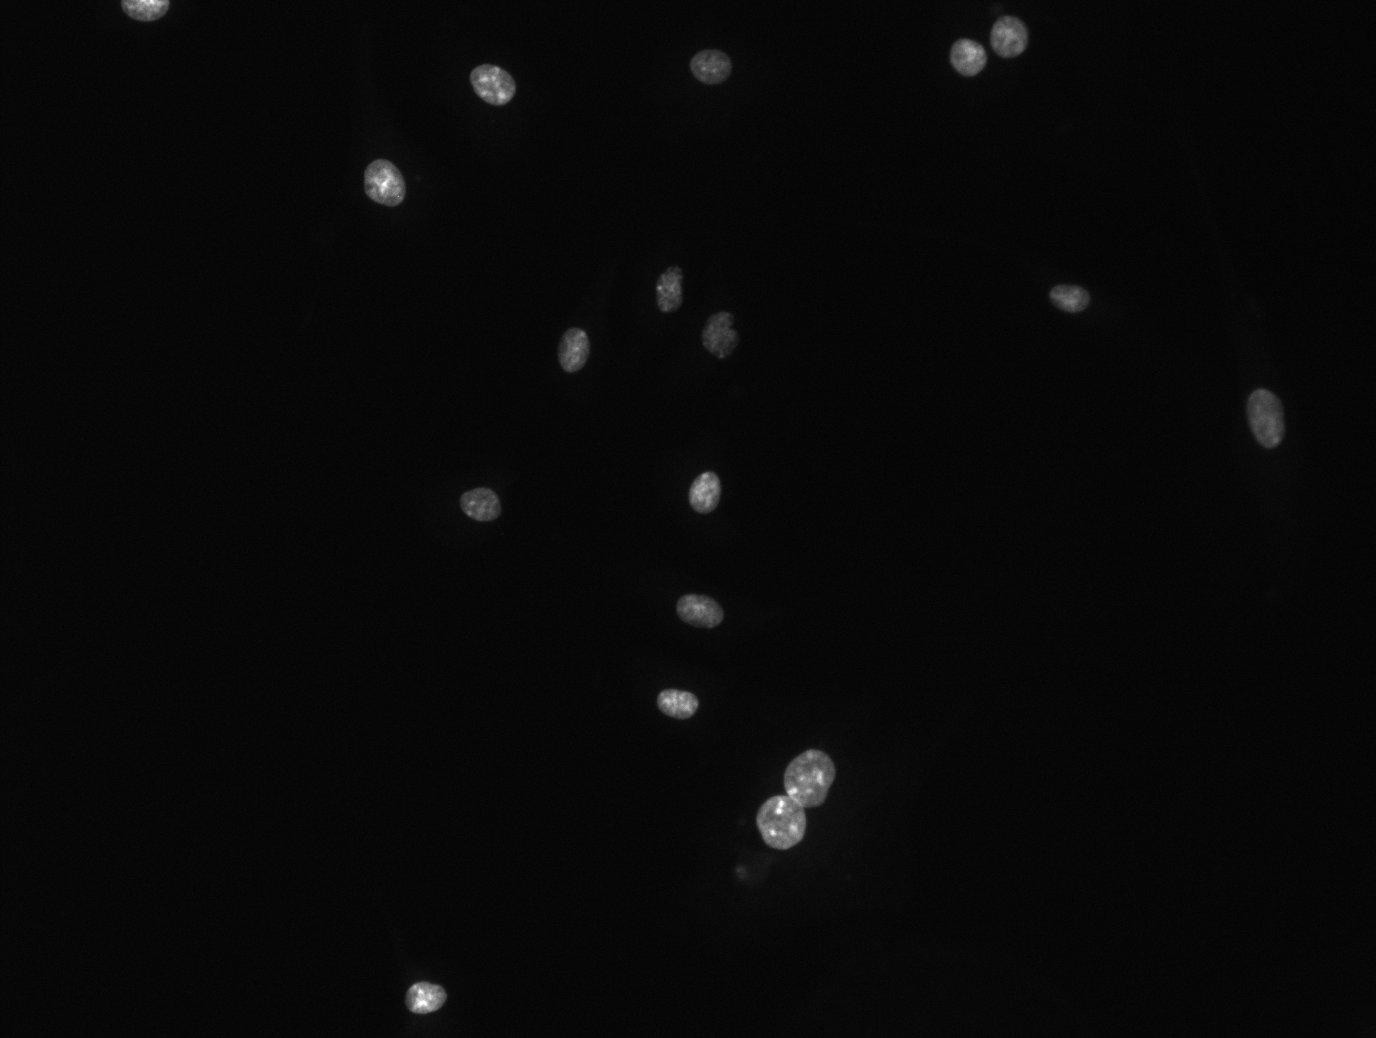
\includegraphics[width = 0.3\linewidth]{Image_2572.jpg} &
			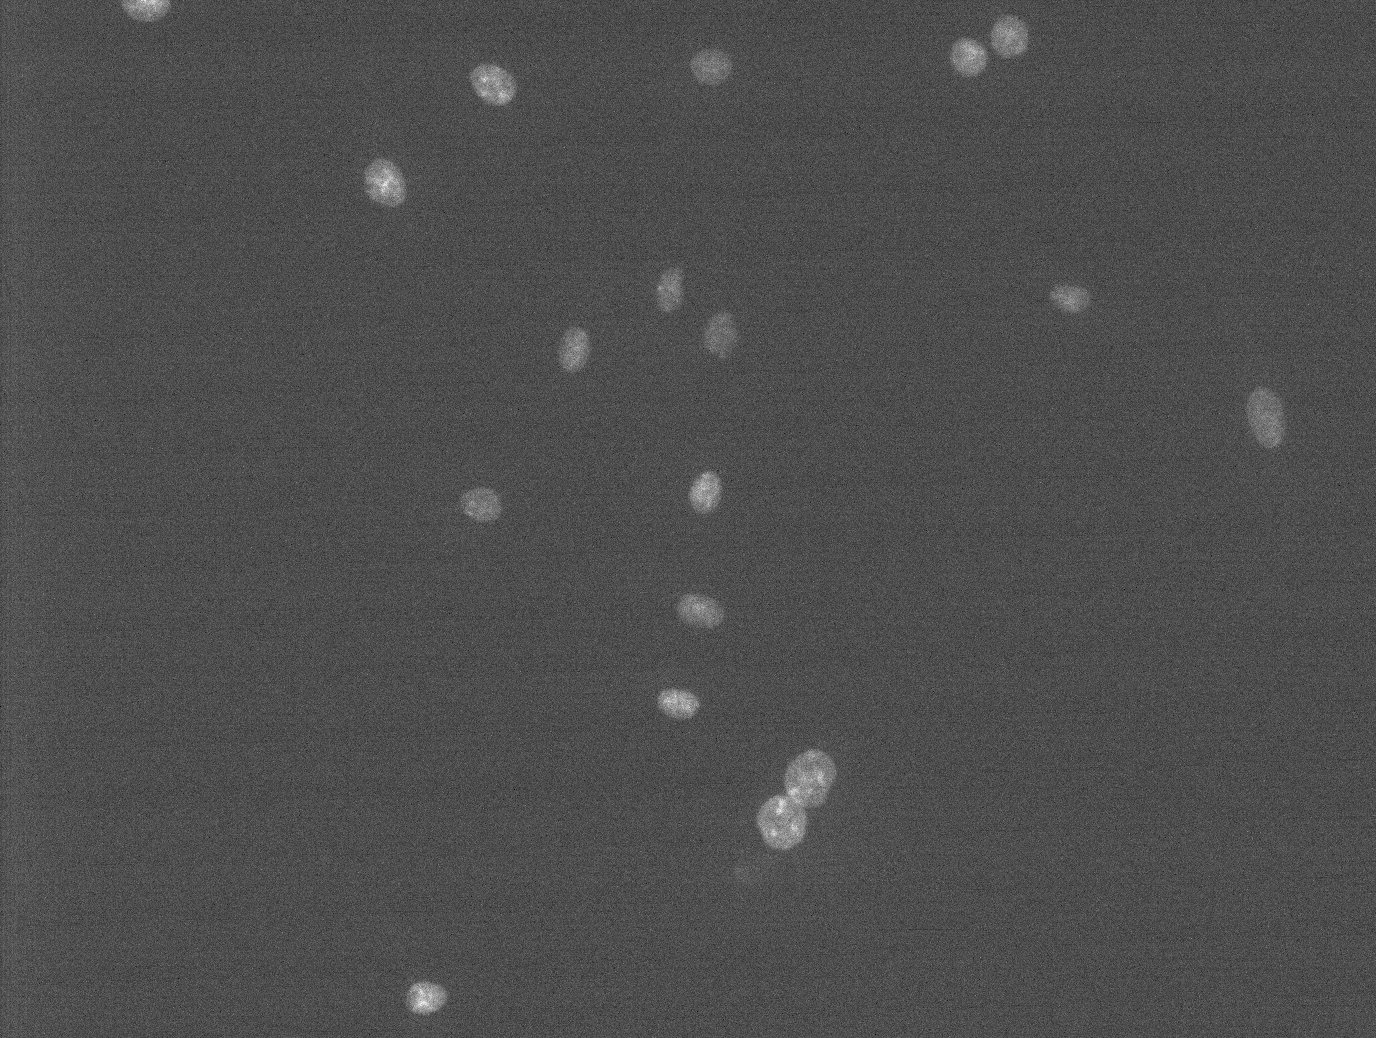
\includegraphics[width = 0.3\linewidth]{Image_2574.jpg}
		\end{tabular}
		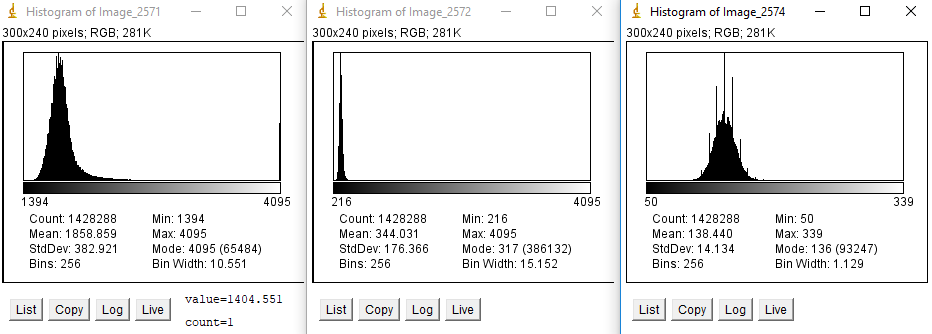
\includegraphics[width=0.9\linewidth]{hists.png}
	\end{figure}
	
	A la izquierda se tiene una imagen saturada, como se observa en el histograma correspondiente existe una densidad de la imagen que se encuentra justo en el límite de los 4095 bits de la cámara, en la imagen central se tiene un buen constraste porque se usa todo la mayor parte del rango dinámico de la cámara, sin embargo si se recorta el rango se observa una disminución en el constraste de las imágenes.
	
	Por esta razón se resalta la importancia de un tiempo de exposición adecuado, si la fotografía se obtiene con sobre exposición la mayoría de los detalles se perderán porque no entra suficiente luz al detector para tenerla encuenta, por el otro lado un exceso de luz satura el detector y no permite obtener información nueva. 
\end{document}
